%\documentclass{beamer}
%\documentclass[c]{beamer}
\documentclass[t]{beamer}
%\documentclass[b]{beamer}
\listfiles

\mode<presentation>
{
% \usetheme[english]{KIT}
% \usetheme[usefoot]{KIT}
  \usetheme[deutsch]{KIT}

%%  \usefonttheme{structurebold}

  \setbeamercovered{transparent}

  %\setbeamertemplate{enumerate items}[circle]
  \setbeamertemplate{enumerate items}[ball]
}

\usepackage{babel}
\date{25.06.2019}
%\DateText

%\KITfoot{\parbox[t]{90mm}{\today:\qquad Dies ist eine sehr lange selbstdefinierte Fu\ss{}zeile -- Dies ist eine sehr lange selbstdefinierte Fu\ss{}zeile -- Dies ist eine sehr lange selbstdefinierte Fu\ss{}zeile}}


\usepackage[utf8]{inputenc}
\usepackage[TS1,T1]{fontenc}
\usepackage{array}
\usepackage{lipsum}
\usepackage{hyperref} 

\usenavigationsymbols
%\usenavigationsymbols[sfHhdb]
%\usenavigationsymbols[sfhHb]

\title[Aufbau einer modernen Rendering-Pipeline]{Aufbau einer modernen Rendering-Pipeline}
\subtitle{Von der Anwendung zum Bildschirm}

\author{Jonas Heinle}

\institute{Fakultät für Informatik - Lehrstuhl für Computergrafik - Institut für Visualisierung und Datenanalyse}

\TitleImage[height=\titleimageht]{Bilder/StormTrooper2Small.png}

\begin{document}

\begin{frame}
  \maketitle
\end{frame}

\section{Anwendung}
\begin{frame}
  \frametitle{Anwendung}
\end{frame}

\section{Geometry Stage}
\begin{frame}
  \frametitle{Primitive Assembly}
\end{frame}

\begin{frame}
  \frametitle{Vertex Shader}

  \begin{centering}
    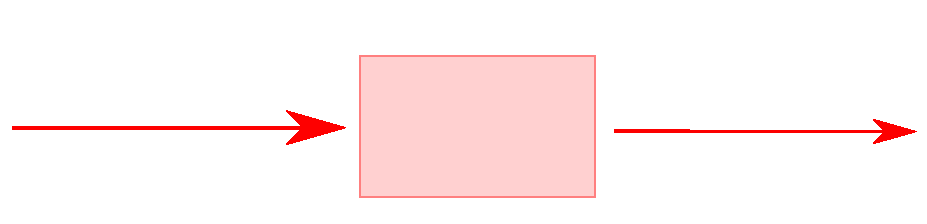
\includegraphics[width=\textwidth]{Bilder/VertexShader.pdf}
  \end{centering}

\end{frame}

\begin{frame}
  \frametitle{Tessellation}

  \begin{centering}
    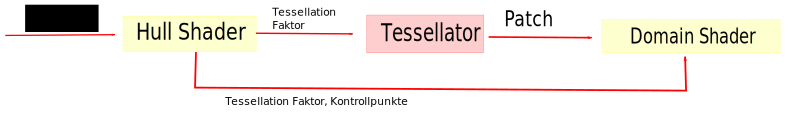
\includegraphics[width=\textwidth]{Bilder/Tessellation.pdf}
  \end{centering}

\end{frame}

\begin{frame}
  \frametitle{Geometry Shader}

  \begin{centering}
    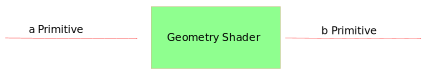
\includegraphics[width=\textwidth]{Bilder/GeometryShader.pdf}
  \end{centering}

\end{frame}

\begin{frame}
  \frametitle{Projektionstransformation}
\end{frame}

\begin{frame}
  \frametitle{Clipping}
\end{frame}

\section{Rasterisierung}
\begin{frame}
  \frametitle{Rasterisierung}

  \begin{centering}
    
\includegraphics[width=\textwidth]{Bilder/Rasterisierung.pdf}
  \end{centering}

\end{frame}

\section{Per Frag Ops}
\begin{frame}
  \frametitle{Per Fragment Operations}
\end{frame}

\section{Compute Shader}
\begin{frame}
  \frametitle{Compute Shader}

  \begin{centering}
    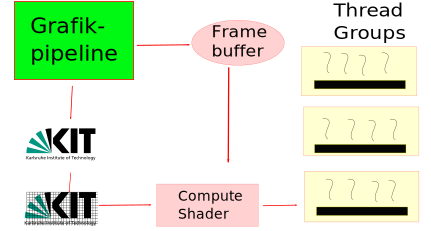
\includegraphics[width=\textwidth]{Bilder/ComputeShader.pdf}
  \end{centering}

\end{frame}

\section{Ausblick}
\begin{frame}
  \frametitle{Raytracing Unterstützung}

  \begin{centering}
    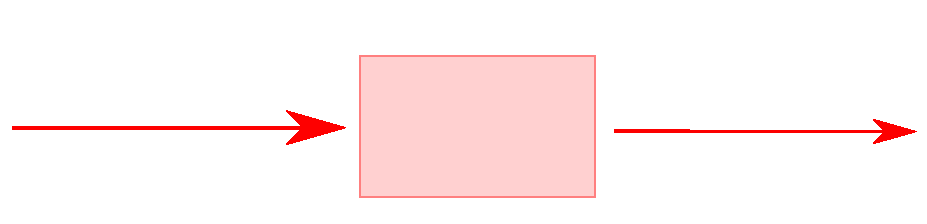
\includegraphics[width=\textwidth]{Bilder/VertexShader.pdf}
  \end{centering}

\end{frame}

\begin{frame}
  \frametitle{Task/-Mesh Shaders}

  \begin{centering}
    \includegraphics[width=\textwidth]{Bilder/geforce-rtx-turing-architecture-mesh-shading-pipeline.png}
  \end{centering}

\end{frame}

\begin{frame}
  \frametitle{Links}
    \heading{Bilder}
    \begin{itemize}
      \item \href{https://arstechnica.com/gaming/2018/03/star-wars-demo-shows-off-just-how-great-real-time-raytracing-can-look/}{Titelbild}
    \end{itemize}
    \bigskip

    \heading{Videos}
  
    \begin{enumerate}
      \item \href{https://www.youtube.com/watch?v=LXo0WdlELJk}{SEED's Project \textit{PICA PICA}}  
      \item \href{https://www.youtube.com/watch?v=CRfZYJ_sk5E}{Nvidias Asteroids Mesh Shaders Demo}
    \end{enumerate}
    
    \vfill
    \mbox{}


\end{frame}

\end{document}
